%\section*{Summary}


\vspace{5mm}
\hrule
\textit{`Much of the variation in healthcare is accounted for by the willingness and ability of doctors to offer treatment rather than differences in illness or patient preference'} John Wennberg, the pioneer of research into clinical variation, and founder of the Dartmouth Atlas of Health Care.
\vspace{2mm}
\hrule

\subsection*{What is the problem?}

Stroke remains one of the leading causes of death and disability, globally and in the UK. The majority of strokes are caused by a clot. Clots may be reduced or removed with \textit{reperfusion} treatments if given soon enough after a stroke. These treatments include thrombolysis, a clot-busting medication given by injection/infusion \cite{emberson_effect_2014} and, more recently, thrombectomy, mechanical removal of a clot performed in a specialist centre \cite{fransen_time_2016}.

Despite thrombolysis being long-established and of proven benefit in ischaemic stroke, use of thrombolysis varies significantly both between hospitals. In England and Wales the national stroke audit reported that in 2021/22, thrombolysis rates for emergency stroke admissions varied from just 1\% to 28\% between hospitals \cite{sentinel_national_stroke_audit_programme_ssnap_2022}, with a median rate of 10.4\%, against a 2019 NHS England long term plan that 20\% of patients of emergency stroke admissions should be receiving thrombolysis. Additionally, in 2022/23, 3.2\% of patients received thrombectomy, significantly below the expected eligibility of at least 10\% \cite{mcmeekin_updating_2021}. 

In addition to variation in outcomes due to disparity in treatment of patients, there is potential for greater use of NHS resources than necessary, as worsened outcomes due to lower use of thrombolysis or thrombectomy can increase downstream healthcare needs.

Figure \ref{fig:flow} shows a summary of the stroke pathway that we model.

\begin{figure}[h!]
\centering
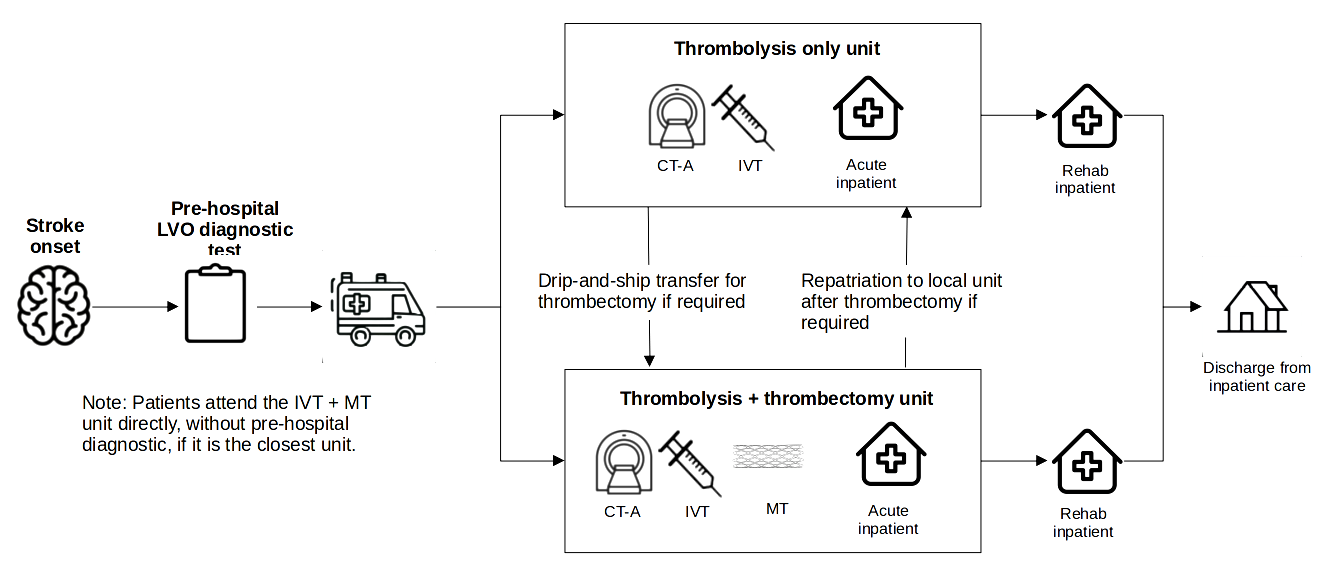
\includegraphics[width=1.0\textwidth]{./images/pathway}
\caption{Summary of patient flow through the emergency and in-patient rehabilitation stroke pathway. Abbreviations used are: LVO = Large Vessel Occlusions (a blockage of a large artery that may be suitable for thrombectomy); IVT = Intravenous Thrombolysis; MT = Mechanical thrombectomy; CT-A = CT-Angiogram (brain scan to confirm the type and location of the stroke).}
\label{fig:flow}
\end{figure}

Our research team uses various modelling techniques, including \textit{explainable machine learning} and \textit{clinical pathway simulation} to identify the variation that occurs across different hospitals during the first few hours of stroke care. We use these models to understand the the source and impact of that variation on patients \cite{allen_using_2022, allen_use_2022}, identifying the variation that comes from hospitals and processes, rather than from differences in local patient populations. We have identified that the majority of between-hospital variation in thrombolysis use comes from differences in hospital processes and decision-making, rather than from differences in local patient populations \cite{allen_using_2022, allen_use_2022}.

We are working with the Sentinel Stroke National Audit Programme and NHS-England on reducing between-hospital variation in emergency stroke care. In this proposed project we will build on previous and existing work, extending the modelling, and bringing it together into a single analysis framework and web application. 

\subsection*{Relevant prior and current work}

\begin{itemize}
    \item \textbf{Geographical analysis} - analysis of variation in access to thrombolysis and thrombectomy \cite{allen_maximising_2019}

    \item \textbf{Thrombolysis pathway and variation in patient selection} - analysis of between-hospital variation in the thrombolysis pathway using clinical pathway simulation and explainable machine learning \cite{allen_use_2022, pearn_what_2023}. Current work, as part of the NIHR SAMueL-2 project \footnote{\url{https://fundingawards.nihr.ac.uk/award/NIHR134326}} is focussing on an analysis of how between-hospital variation in selection of patients for thrombolysis affects patient outcomes. This work has produced a web tool \footnote{\url{https://stroke-predictions.streamlit.app/}}, including a health economics model. The tool is being used in a project with NHS-England and the national stroke audit, to facilitate improvement in thrombolysis use in lower thrombolysing units. 

    \item \textbf{Pre-hospital pathway} - As part of the NIHR OptImIST programme \footnote{\url{https://fundingawards.nihr.ac.uk/award/NIHR202361}}, we are modelling the effect of pre-hopsital selection of patients for thrombectomy. We model how pre-hospital selection of patients for thrombectomy will the effect time to thrombolysis and thrombectomy, and their outcomes (using a mathematical outcome model based on time to treatment).
    
\end{itemize}

\subsection*{Proposed work}

We wish to extend our current work in the following ways:

\begin{itemize}

    \item \textbf{Wake-up and late-presenting stroke} - updating our existing models to align with new clinical guidelines that thrombolysis should be considered up to 9 hours for late-presenting and wake-up stroke patients, after advanced imaging for an assessment of whether there is still salvageable brain tissue.
    
    \item \textbf{Analysis of variation in patient selection for thrombectomy} - how do thrombectomy centres vary in their selection of patients for thrombectomy, and what is the likely effect on outcomes from this variation?

    \item \textbf{Analysis of how variation in use of thrombolysis and thrombectomy effects in-patient length of stay} - how do thrombolysis and thrombectomy affect length of stay in acute and rehabilitation units?

    \item \textbf{Causal inference studies} - are observations from predictive models supported by causal inference studies, testing that any predictions made can be attributed to the assumed cause?

    \item \textbf{Production of a combined analytical pathway and web tool} - this tool will provide a national and regional analysis of current thrombolysis and thrombectomy use and provision, and enable an understanding of what an optimal system may look like, and the effect that would have on patients and health services. The tool will be developed and refined with co-production workshops, as we work with stroke teams on local thrombolysis and thrombectomy improvement. The web tool will combine:
    
    \begin{enumerate}
        \item Geographical analysis of access to thrombolysis and thrombectomy. The map will identify which destination hospital would provide most likely best outcome depending on type of stroke (or if stroke type is unknown)

        \item Clinical pathway simulation (including the pre-hospital pathway) - showing how optimisation of the pathway may affect thrombolysis and thrombectomy use and speed.

        \item Explainable machine-learning analysis of variation in choice of patients for thrombolysis and thrombectomy (with causal inference methodology to give further confidence in modelling).

        \item A health economics model based on patient outcomes, extending patient outcome results to expected QALY (quality-adjusted life years).
    \end{enumerate} 
    
\end{itemize}

